During validation of the final end-of-year reprocessing of the 2015 data, a misalignment was found in the barrel of the TRT detector, as several modules (triangular clusters of straws) showed rotations in the local $y$ coordinate.
The then-best available constants included a full L3 alignment of the silicon detectors and a separate L2 alignment of the TRT.
However, not all degrees of freedom were enabled when the TRT was aligned.
To correct for these tilts, an additional four iterations of L2 alignment TRT was performed on the TRT enabling all available degrees of freedom ($T_x$, $T_y$, $R_x$, $R_y$, and $R_z$ in the barrel, and $T_x$, $T_y$, and $R_z$ for the endcaps).
Plots of the residual means from barrel $\phi$ sectors containing modules affected by the tilt misalignment are shown in Figure~\ref{fig:align_trt_l2} before and after the L2 alignment.

\begin{figure}[htbp]
  \centering
  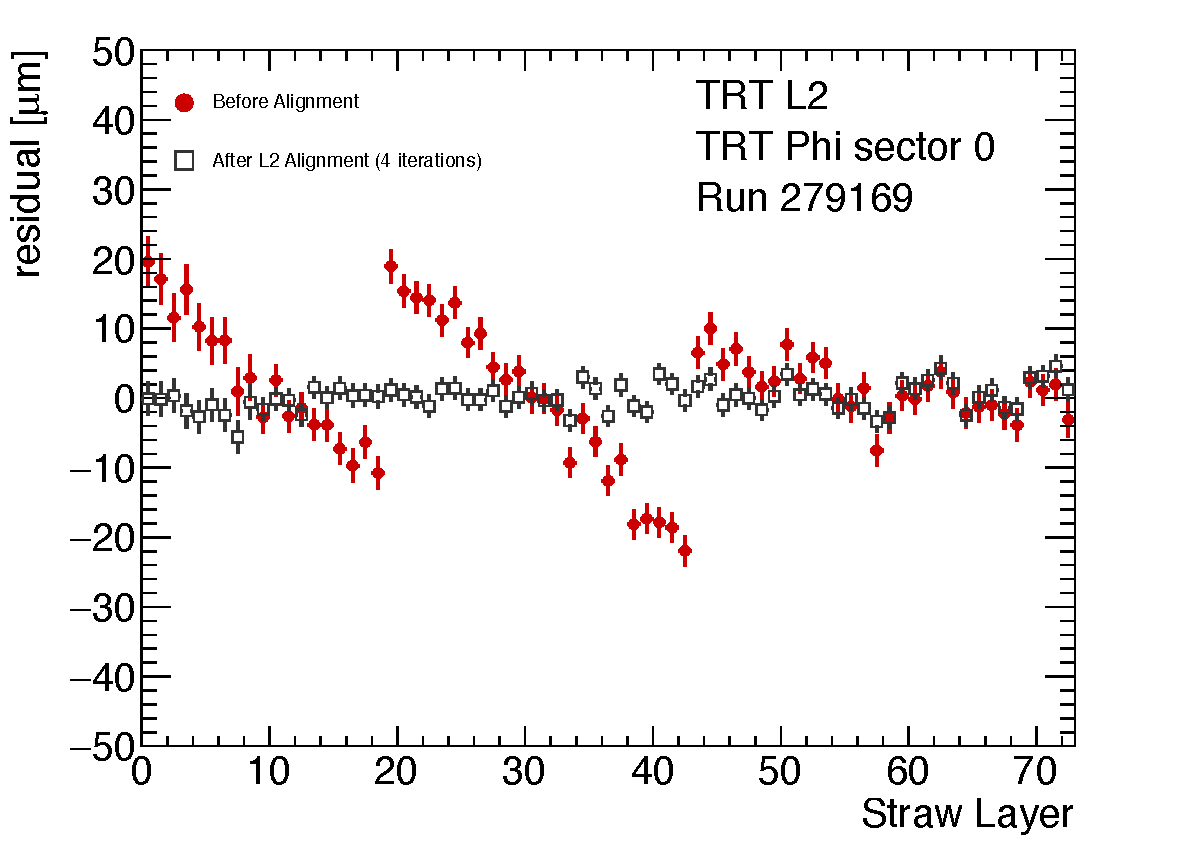
\includegraphics[width=.48\textwidth]{figs/alignment/trt/TRT_aveResVsStrawLayerModule0}
  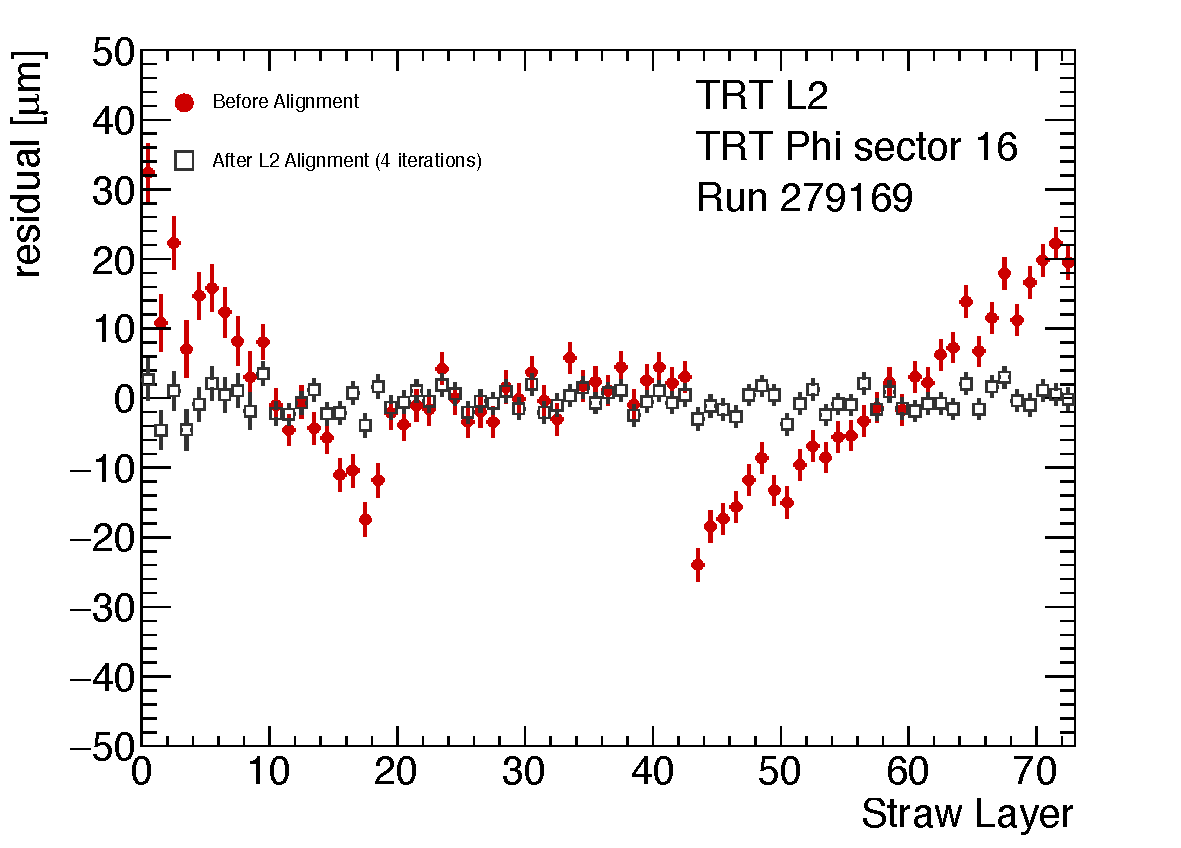
\includegraphics[width=.48\textwidth]{figs/alignment/trt/TRT_aveResVsStrawLayerModule16}
  \caption{Residual means by straw layer in two TRT $\phi$-sectors affected by a tilt misalignment.  The tilts in each of the three modules are clearly visible in the red points representing the reconstructed data prior to alignment.  After four iterations of L2 alignment, the residual means in the gray points are flat.}
  \label{fig:align_trt_l2}
\end{figure}

Following the L2 alignment, some additional time was taken to determine if a full wire-by-wire L3 alignment of the TRT was necessary.
The TRT was last aligned at L3 during Run 1, but initial alignment campaigns in Run 2 did not show signs of misalignment, as can be seen from the residual distributions in Figure~\ref{fig:align_2015_results_trt}.
In order to assess the alignment more carefully, two dimensional residual maps in $\phi$ and $z$ were constructed for each layer in the TRT barrel and endcaps using the current alignment.
These maps were compared to a similar set using the L3 alignment from 2010, from which it was determined that the straw-level alignment indeed hadn't degraded and a new L3 alignment was not needed.
The maps for the first layer of the TRT barrel are shown in Figure~\ref{fig:align_trt_map} for both sets of alignment constants.


\begin{figure}[htbp]
  \centering
  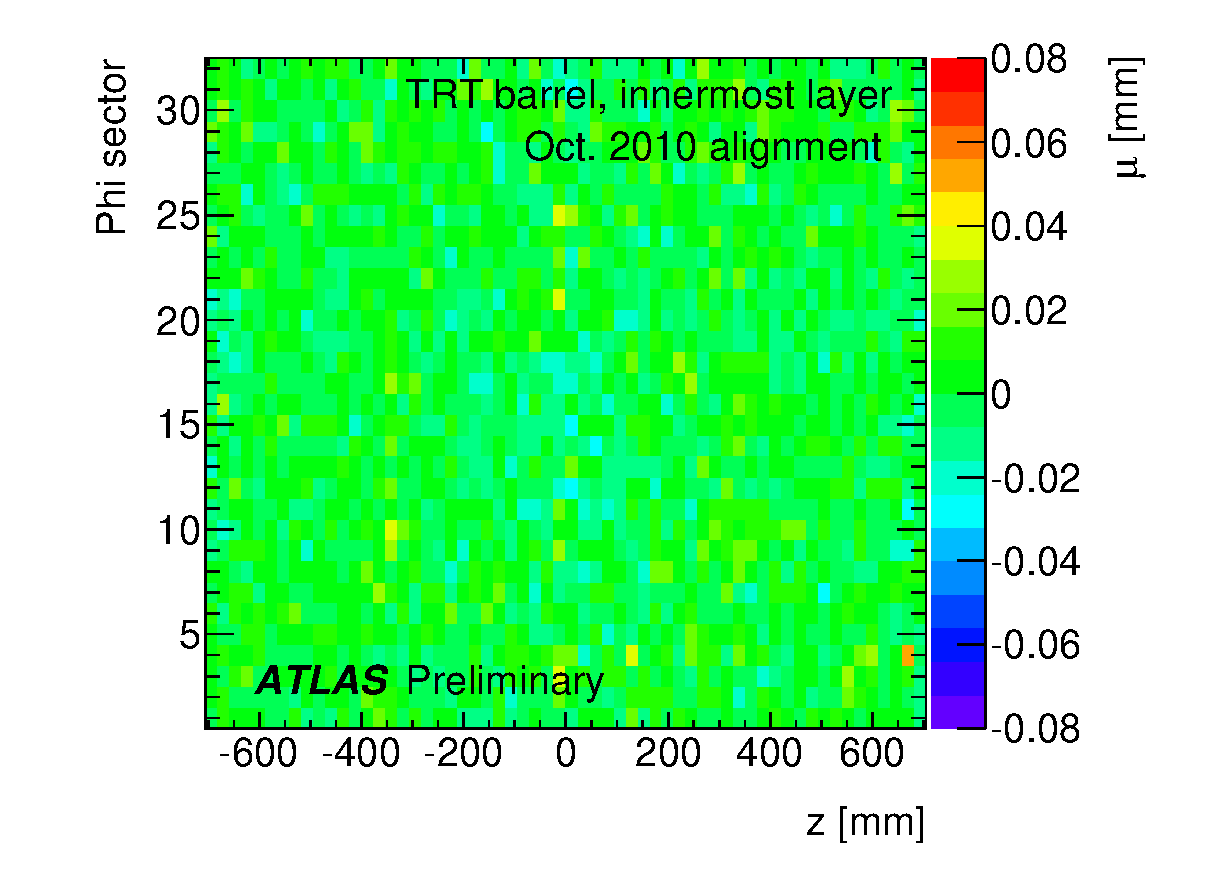
\includegraphics[height=.25\textheight]{figs/alignment/trt/TRT_barrel_ResMaps_Oct10}
  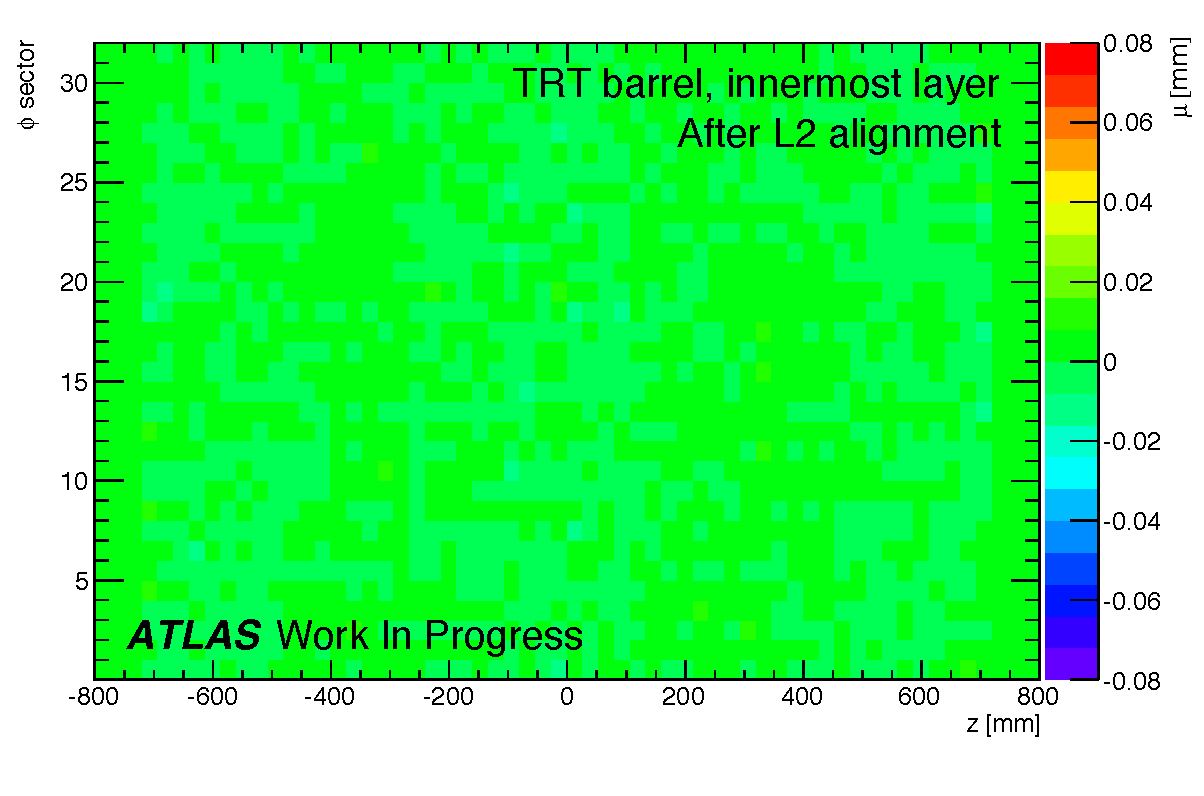
\includegraphics[height=.25\textheight]{figs/alignment/trt/trt_b_aveResVsPhiZ_l0_compare}
  \caption[Two dimensional map of residuals in the first layer of the TRT barrel vs $z$ and $\phi$.  Each bin represents the mean of a Gaussian fit to the TRT residuals in that bin.  The map on the left is after the L3 (wire-by-wire) alignment of the TRT performed in 2010, and the map on the right is after the L2 alignment at the end of 2015.  The $z$-axis for both plots use the same scale.]{Two dimensional map of residuals in the first layer of the TRT barrel vs $z$ and $\phi$.  Each bin represents the mean of a Gaussian fit to the TRT residuals in that bin.  The map on the left is after the L3 (wire-by-wire) alignment of the TRT performed in 2010, and the map on the right is after the L2 alignment at the end of 2015.  The $z$-axis for both plots use the same scale.  Left figure taken from~\cite{2011.alignment-7tev}.}
  \label{fig:align_trt_map}
\end{figure}
